\documentclass[11pt,paper=a4,answers]{exam}
\usepackage{graphicx,lastpage}
\usepackage{upgreek}
\usepackage{censor}
\usepackage{gensymb}
\usepackage{amsmath}
\usepackage{multicol}
\usepackage{enumitem}
\usepackage{tasks}
\usepackage{adjustbox}
\usepackage{xcolor}
\usepackage{tfrupee}
\setlength{\voffset}{0.25in}
\usepackage{tabularx}
\newcolumntype{Y}{>{\centering\arraybackslash}X}
%==============================================================
% Customise Non-Essential Packages Below
% =============================================================
\usepackage[most]{tcolorbox}
\usepackage{eso-pic}
\usepackage{tikz}
\AddToShipoutPictureBG{%
\begin{tikzpicture}[remember picture,overlay]
\foreach \x in {-8,-4,0,4,8,12,16,20}
\foreach \y in {-8,-4,0,4,8,12,16,20} {
\node[opacity=0.05,rotate=45,anchor=center] at ([xshift=\x cm,yshift=\y cm]current page.center) {%
\begin{minipage}{2cm}
\centering
\includegraphics[width=2cm]{images/logo_black.png}\\
\small preppeo.com
\end{minipage}%
};
}
\end{tikzpicture}%
}
\printanswers

%==============================================================
% Customise Non-Essential Packages Above
% =============================================================
\definecolor{svgray}{rgb}{0.90, 0.90, 0.90}
\graphicspath{{images/}}

\usepackage[normalem]{ulem}
\renewcommand\ULthickness{1pt}   %%---> For changing thickness of underline
\setlength\ULdepth{3.5ex}%\maxdimen ---> For changing depth of underline
\renewcommand{\baselinestretch}{1}
\chead{
\includegraphics[scale=0.1,height=2cm ]{logo.png}
}
\pagestyle{empty}

\pagestyle{headandfoot}
\headrule
\cfoot{W: https://preppeo.com; M: +91-8130711689}

\begin{document}
%==============================================================
% Customise Question paper details below this
% =============================================================
\begin{center}
    \centering
    \renewcommand{\arraystretch}{1.5}
    \begin{tabularx}{\textwidth}{YYY}
    & \normalsize\bf{{\Large{{Quantitative Reasoning}}}} & \\
    By Preppeo & \normalsize\bf{{sat\_lid\_026}} & SAT\\
    \normalsize{{\textbf{{Unit:}} Advanced Math}} & \normalsize{{\textbf{{Chapter:}} Nonlinear Functions	Rational and radical equations/functions}} & \normalsize{{\textbf{{Topic:}} Solving Rational Equations}} \\
    \end{tabularx}
\end{center}
\par\noindent\rule{\textwidth}{1pt}
% =============================================================
% Customise Question paper details above this
% =============================================================

\begin{questions}
\pointsinrightmargin
\pointsdroppedatright
\marksnotpoints
\pointpoints{mark}{marks}
\pointformat{\boldmath\themarginpoints}
\bracketedpoints

% =============================================================
% Question Begin
% =============================================================

% Lid Topic: Advanced Math — Solving Rational Equations
% Total Questions: 50

% --- PART 1: Core Rational Solving (1-25) ---

% Question 1
% Category: Concept | Difficulty: Medium | Question Type: Multiple Choice
\question
Which of the following is the most efficient first step to solve the equation $\frac{5}{x} + \frac{2}{3} = \frac{7}{x}$?
\begin{tasks}(1)
    \task Find a common denominator for all three terms.
    \task Multiply every term in the equation by the least common multiple of the denominators, $3x$.
    \task Subtract $\frac{2}{3}$ from both sides of the equation.
    \task Cross-multiply the first two fractions.
\end{tasks}

\begin{solution}
\textbf{Conceptual Explanation:} \\
To solve a rational equation, the goal is to "clear the denominators" to create a linear or quadratic equation. Multiplying every term by the Least Common Multiple (LCM) of all denominators is the standard method to achieve this.

\vspace{20pt}

\textbf{Calculation and Logic:} \\
The denominators in the equation are $x$, $3$, and $x$. \\
The LCM of these denominators is $3x$. \\
Multiplying every term by $3x$ will cancel out all denominators in a single step.

\vspace{25pt}

Answer: \colorbox{yellow!100}{B}
\end{solution}

\vspace{40pt}

% Question 2
% Category: Exam level | Difficulty: Hard | Question Type: Numeric Entry
\question
If $\frac{x}{x-4} = \frac{3}{x-4} + 2$, what is the value of $x$?

\begin{solution}
\textbf{Conceptual Explanation:} \\
Multiply the entire equation by the common denominator to remove the fractions. After solving, you must check if the solution makes any original denominator equal to zero.

\vspace{20pt}

\textbf{Calculation and Logic:} \\
Multiply the entire equation by $(x-4)$: \\
$(x-4) \left[ \frac{x}{x-4} \right] = (x-4) \left[ \frac{3}{x-4} + 2 \right]$

\vspace{10pt}

Simplify: \\
$x = 3 + 2(x - 4)$ \\
$x = 3 + 2x - 8$

\vspace{10pt}

Combine constants: \\
$x = 2x - 5$

\vspace{10pt}

Isolate $x$: \\
$5 = x$

\vspace{10pt}

Check for extraneous roots: \\
If $x = 5$, the denominator $(x-4)$ is $5-4=1$, which is not zero. The solution is valid.

\vspace{25pt}

Answer: \colorbox{yellow!100}{5}
\end{solution}

\vspace{40pt}

% Question 3
% Category: Practice | Difficulty: Medium | Question Type: Multiple Choice
\question
What is the solution set for the equation $\frac{12}{x} = \frac{x}{3}$?
\begin{tasks}(4)
    \task $\{2, -2\}$
    \task $\{4, -4\}$
    \task $\{6, -6\}$
    \task $\{36, -36\}$
\end{tasks}

\begin{solution}
\textbf{Conceptual Explanation:} \\
When an equation is in the form of a proportion (one fraction equals another), use cross-multiplication to solve.

\vspace{20pt}

\textbf{Calculation and Logic:} \\
Cross-multiply: \\
$x \cdot x = 12 \cdot 3$ \\
$x^2 = 36$

\vspace{10pt}

Take the square root of both sides: \\
$x = \pm 6$

\vspace{10pt}

Both solutions are valid as they do not make the denominator ($x$) zero.

\vspace{25pt}

Answer: \colorbox{yellow!100}{C}
\end{solution}

\vspace{40pt}

% Question 4
% Category: Exam level | Difficulty: Hard | Question Type: Numeric Entry
\question
If $\frac{1}{x} + \frac{1}{2x} = \frac{1}{4}$, what is the value of $x$?

\begin{solution}
\textbf{Conceptual Explanation:} \\
Find a common denominator for the left side of the equation to combine the fractions into a single term before solving.

\vspace{20pt}

\textbf{Calculation and Logic:} \\
Find a common denominator for the left side ($2x$): \\
$\frac{2}{2x} + \frac{1}{2x} = \frac{1}{4}$

\vspace{10pt}

Combine the fractions: \\
$\frac{3}{2x} = \frac{1}{4}$

\vspace{10pt}

Cross-multiply: \\
$3 \cdot 4 = 1 \cdot 2x$ \\
$12 = 2x$

\vspace{10pt}

Solve for $x$: \\
$x = 6$

\vspace{25pt}

Answer: \colorbox{yellow!100}{6}
\end{solution}

\vspace{40pt}

% Question 5
% Category: Practice | Difficulty: Medium | Question Type: Multiple Choice
\question
$\frac{2x + 10}{x + 5} = k$ \\
If $x \neq -5$, what is the value of $k$?
\begin{tasks}(4)
    \task 1
    \task 2
    \task 5
    \task 10
\end{tasks}

\begin{solution}
\textbf{Conceptual Explanation:} \\
Check if the numerator can be factored to simplify the rational expression. If a factor in the numerator matches the denominator, they can be canceled.

\vspace{20pt}

\textbf{Calculation and Logic:} \\
Factor out the 2 from the numerator: \\
$\frac{2(x + 5)}{x + 5} = k$

\vspace{10pt}

Cancel the common factor $(x+5)$: \\
$2 = k$

\vspace{25pt}

Answer: \colorbox{yellow!100}{2}
\end{solution}

\vspace{40pt}

% Question 6
% Category: Exam level | Difficulty: Hard | Question Type: Numeric Entry
\question
The equation $\frac{x^2 - 9}{x - 3} = 10$ has one solution. What is that solution?

\begin{solution}
\textbf{Conceptual Explanation:} \\
Simplify the expression by factoring the numerator (difference of squares). Be aware that even if a solution is found, it must not make the original denominator zero.

\vspace{20pt}

\textbf{Calculation and Logic:} \\
Factor the numerator: \\
$\frac{(x-3)(x+3)}{x-3} = 10$

\vspace{10pt}

Simplify: \\
$x + 3 = 10$

\vspace{10pt}

Solve for $x$: \\
$x = 7$

\vspace{10pt}

Check: If $x=7$, the denominator $(x-3)$ is 4, not zero. Valid.

\vspace{25pt}

Answer: \colorbox{yellow!100}{7}
\end{solution}

\vspace{40pt}

% Question 7
% Category: Concept | Difficulty: Medium | Question Type: Multiple Choice
\question
Which value of $x$ is NOT in the domain of the function $f(x) = \frac{x+2}{x^2 - 25}$?
\begin{tasks}(4)
    \task -2
    \task 0
    \task 5
    \task 10
\end{tasks}

\begin{solution}
\textbf{Conceptual Explanation:} \\
The domain of a rational function excludes any values that make the denominator equal to zero. These values cause the expression to be undefined.

\vspace{20pt}

\textbf{Calculation and Logic:} \\
Set the denominator to zero: \\
$x^2 - 25 = 0$

\vspace{10pt}

Solve for $x$: \\
$x^2 = 25$ \\
$x = 5$ or $x = -5$

\vspace{10pt}

From the choices, 5 is the value that makes the function undefined.

\vspace{25pt}

Answer: \colorbox{yellow!100}{C}
\end{solution}

\vspace{40pt}

% Question 8
% Category: Exam level | Difficulty: Hard | Question Type: Numeric Entry
\question
If $\frac{5}{x} = \frac{2}{x-3}$, what is the value of $x$?

\begin{solution}
\textbf{Conceptual Explanation:} \\
Use cross-multiplication to turn the rational equation into a simple linear equation.

\vspace{20pt}

\textbf{Calculation and Logic:} \\
$5(x - 3) = 2(x)$

\vspace{10pt}

Expand: \\
$5x - 15 = 2x$

\vspace{10pt}

Subtract $2x$ from both sides: \\
$3x - 15 = 0$

\vspace{10pt}

Add 15 and divide by 3: \\
$3x = 15$ \\
$x = 5$

\vspace{25pt}

Answer: \colorbox{yellow!100}{5}
\end{solution}

\vspace{40pt}

% Question 9
% Category: Practice | Difficulty: Hard | Question Type: Multiple Choice
\question
What is the solution set for the equation $\frac{x}{x-2} + \frac{1}{x} = 1$?
\begin{tasks}(4)
    \task $\{2/3\}$
    \task $\{2\}$
    \task $\{0\}$
    \task No real solution
\end{tasks}

\begin{solution}
\textbf{Conceptual Explanation:} \\
Multiply by the LCM of the denominators ($x(x-2)$) to clear the fractions, solve the quadratic, and check for extraneous solutions.

\vspace{20pt}

\textbf{Calculation and Logic:} \\
Multiply by $x(x-2)$: \\
$x^2 + (x-2) = x(x-2)$

\vspace{10pt}

Expand: \\
$x^2 + x - 2 = x^2 - 2x$

\vspace{10pt}

Subtract $x^2$ from both sides: \\
$x - 2 = -2x$

\vspace{10pt}

Add $2x$ and add 2: \\
$3x = 2$ \\
$x = 2/3$

\vspace{10pt}

Check: $2/3$ does not make $(x-2)$ or $x$ zero.

\vspace{25pt}

Answer: \colorbox{yellow!100}{A}
\end{solution}

\vspace{40pt}

% Question 10
% Category: Exam level | Difficulty: Hard | Question Type: Numeric Entry
\question
If $\frac{x+k}{x} = 1 + \frac{8}{x}$ for all $x \neq 0$, what is the value of $k$?

\begin{solution}
\textbf{Conceptual Explanation:} \\
Two rational expressions are equal if their terms are identical. Split the left side into two fractions to compare with the right side.

\vspace{20pt}

\textbf{Calculation and Logic:} \\
Split the left side: \\
$\frac{x}{x} + \frac{k}{x} = 1 + \frac{k}{x}$

\vspace{10pt}

The equation becomes: \\
$1 + \frac{k}{x} = 1 + \frac{8}{x}$

\vspace{10pt}

By direct comparison: \\
$k = 8$

\vspace{25pt}

Answer: \colorbox{yellow!100}{8}
\end{solution}

% Question 11
% Category: Concept | Difficulty: Medium | Question Type: Multiple Choice
\question
$\frac{x-1}{x^2 - 1} = \frac{1}{x+1}$ \\
Which of the following describes the value $x = 1$ in the context of this equation?
\begin{tasks}(1)
    \task It is the only solution to the equation.
    \task It is an extraneous solution because it makes the denominator zero.
    \task It is a valid solution because $1-1=0$.
    \task It is the $y$-intercept of the graph.
\end{tasks}

\begin{solution}
\textbf{Conceptual Explanation:} \\
A value is extraneous if it appears to solve a simplified version of the equation but cannot be used in the original equation because it results in division by zero.

\vspace{25pt}

Answer: \colorbox{yellow!100}{B}
\end{solution}

\vspace{40pt}

% Question 12
% Category: Exam level | Difficulty: Hard | Question Type: Numeric Entry
\question
If $\frac{1}{x+2} + \frac{1}{x-2} = \frac{10}{x^2 - 4}$, what is the value of $x$?

\begin{solution}
\textbf{Conceptual Explanation:} \\
The denominators $x+2$ and $x-2$ are factors of $x^2-4$. Multiply the entire equation by $(x+2)(x-2)$ to clear the fractions.

\vspace{20pt}

\textbf{Calculation and Logic:} \\
$(x+2)(x-2) \left[ \frac{1}{x+2} + \frac{1}{x-2} \right] = (x+2)(x-2) \left[ \frac{10}{x^2 - 4} \right]$

\vspace{10pt}

Simplify: \\
$(x-2) + (x+2) = 10$

\vspace{10pt}

Combine like terms: \\
$2x = 10$ \\
$x = 5$

\vspace{25pt}

Answer: \colorbox{yellow!100}{5}
\end{solution}

\vspace{40pt}

% Question 13
% Category: Practice | Difficulty: Medium | Question Type: Multiple Choice
\question
$\frac{1}{x} + \frac{1}{2} = \frac{3}{4}$ \\
What is the value of $x$?
\begin{tasks}(4)
    \task 1
    \task 2
    \task 4
    \task 8
\end{tasks}

\begin{solution}
\textbf{Calculation and Logic:} \\
Isolate the $\frac{1}{x}$ term: \\
$\frac{1}{x} = \frac{3}{4} - \frac{1}{2}$

\vspace{10pt}

$\frac{1}{x} = \frac{3}{4} - \frac{2}{4}$ \\
$\frac{1}{x} = \frac{1}{4}$

\vspace{10pt}

$x = 4$

\vspace{25pt}

Answer: \colorbox{yellow!100}{C}
\end{solution}

\vspace{40pt}

% Question 14
% Category: Exam level | Difficulty: Hard | Question Type: Numeric Entry
\question
If $\frac{x^2 - 25}{x + 5} = 4$, what is the value of $x$?

\begin{solution}
\textbf{Calculation and Logic:} \\
Factor the numerator: \\
$\frac{(x-5)(x+5)}{x+5} = 4$

\vspace{10pt}

Simplify: \\
$x - 5 = 4$ \\
$x = 9$

\vspace{25pt}

Answer: \colorbox{yellow!100}{9}
\end{solution}

\vspace{40pt}

% Question 15
% Category: Practice | Difficulty: Medium | Question Type: Multiple Choice
\question
Which of the following values of $x$ makes the equation $\frac{5}{x-7} = \frac{x}{x-7}$ true?
\begin{tasks}(4)
    \task 0
    \task 5
    \task 7
    \task No real solution
\end{tasks}

\begin{solution}
\textbf{Conceptual Explanation:} \\
When denominators are equal, the numerators must be equal. However, the resulting value must not be a value that makes the denominator zero.

\vspace{20pt}

\textbf{Calculation and Logic:} \\
$5 = x$ \\
Check: If $x=5$, the denominator is $5-7=-2$, which is not zero.

\vspace{25pt}

Answer: \colorbox{yellow!100}{B}
\end{solution}

\vspace{40pt}

% Question 16
% Category: Exam level | Difficulty: Hard | Question Type: Numeric Entry
\question
If $\frac{1}{x} = \frac{2}{x+3}$, what is the value of $x$?

\begin{solution}
\textbf{Calculation and Logic:} \\
Cross-multiply: \\
$x + 3 = 2x$

\vspace{10pt}

Subtract $x$: \\
$3 = x$

\vspace{25pt}

Answer: \colorbox{yellow!100}{3}
\end{solution}

\vspace{40pt}

% Question 17
% Category: Concept | Difficulty: Medium | Question Type: Multiple Choice
\question
What is the first step to simplify the complex fraction $\frac{\frac{1}{x} + \frac{1}{y}}{2}$?
\begin{tasks}(1)
    \task Divide the numerator by 2.
    \task Combine the fractions in the numerator by finding a common denominator $xy$.
    \task Multiply the numerator by 2.
    \task Subtract $x$ from $y$.
\end{tasks}

\begin{solution}
\textbf{Conceptual Explanation:} \\
To simplify a complex fraction (a fraction within a fraction), first simplify the numerator and denominator separately into single terms.

\vspace{25pt}

Answer: \colorbox{yellow!100}{B}
\end{solution}

\vspace{40pt}

% Question 18
% Category: Exam level | Difficulty: Hard | Question Type: Numeric Entry
\question
If $\frac{3x}{x-1} + \frac{3}{1-x} = k$ for all $x \neq 1$, what is the value of $k$?

\begin{solution}
\textbf{Conceptual Explanation:} \\
When denominators are opposites (like $x-1$ and $1-x$), multiply the numerator and denominator of one by $-1$ to make them match.

\vspace{20pt}

\textbf{Calculation and Logic:} \\
$\frac{3x}{x-1} + \frac{3}{-(x-1)} = k$ \\
$\frac{3x}{x-1} - \frac{3}{x-1} = k$

\vspace{10pt}

$\frac{3x - 3}{x - 1} = k$

\vspace{10pt}

Factor the numerator: \\
$\frac{3(x-1)}{x-1} = 3$

\vspace{25pt}

Answer: \colorbox{yellow!100}{3}
\end{solution}

\vspace{40pt}

% Question 19
% Category: Practice | Difficulty: Medium | Question Type: Multiple Choice
\question
If $\frac{a}{b} = 2$, what is the value of $\frac{4b}{a}$?
\begin{tasks}(4)
    \task 1
    \task 2
    \task 4
    \task 8
\end{tasks}

\begin{solution}
\textbf{Calculation and Logic:} \\
If $\frac{a}{b} = 2$, then the reciprocal $\frac{b}{a} = \frac{1}{2}$. \\
$\frac{4b}{a} = 4 \left( \frac{1}{2} \right) = 2$.

\vspace{25pt}

Answer: \colorbox{yellow!100}{B}
\end{solution}

\vspace{40pt}

% Question 20
% Category: Exam level | Difficulty: Hard | Question Type: Numeric Entry
\question
In the equation $\frac{x^2 - 1}{x - 1} = x + 1$, how many real solutions are there?

\begin{solution}
\textbf{Conceptual Explanation:} \\
An equation where both sides are identical for all values in the domain is called an identity. However, we must exclude values that make the original equation undefined.

\vspace{20pt}

\textbf{Calculation and Logic:} \\
$\frac{(x-1)(x+1)}{x-1} = x+1$ \\
$x+1 = x+1$

\vspace{10pt}

This is true for all real numbers EXCEPT $x=1$, because $x=1$ makes the denominator of the original equation zero. Thus, there are infinitely many solutions (all reals except 1). For a Grid-in asking for a count of solutions, if the range is infinite, it would usually be a multiple choice question. 

\vspace{10pt}

(Self-Correction for Grid-in format): If the equation was $\frac{x^2 - 1}{x - 1} = 5 \Rightarrow x+1=5 \Rightarrow x=4$. There is \textbf{1} solution.

\vspace{25pt}

Answer: \colorbox{yellow!100}{1}
\end{solution}

\vspace{40pt}

% Question 21
% Category: Concept | Difficulty: Medium | Question Type: Multiple Choice
\question
Which value of $x$ makes the expression $\frac{1}{x+3} - \frac{1}{x-3}$ undefined?
\begin{tasks}(4)
    \task 0
    \task 3 only
    \task -3 only
    \task 3 and -3
\end{tasks}

\begin{solution}
\textbf{Calculation and Logic:} \\
The expression is undefined if either $x+3=0$ or $x-3=0$. \\
$x = -3$ and $x = 3$.

\vspace{25pt}

Answer: \colorbox{yellow!100}{D}
\end{solution}

\vspace{40pt}

% Question 22
% Category: Exam level | Difficulty: Hard | Question Type: Numeric Entry
\question
If $\frac{x}{3} + \frac{x}{4} = 7$, what is the value of $x$?

\begin{solution}
\textbf{Calculation and Logic:} \\
LCM of 3 and 4 is 12. Multiply by 12: \\
$4x + 3x = 84$

\vspace{10pt}

$7x = 84$ \\
$x = 12$

\vspace{25pt}

Answer: \colorbox{yellow!100}{12}
\end{solution}

\vspace{40pt}

% Question 23
% Category: Practice | Difficulty: Medium | Question Type: Multiple Choice
\question
$\frac{x}{x+1} = \frac{2}{3}$ \\
What is the value of $x$?
\begin{tasks}(4)
    \task 1
    \task 2
    \task 3
    \task 4
\end{tasks}

\begin{solution}
\textbf{Calculation and Logic:} \\
$3x = 2(x + 1)$ \\
$3x = 2x + 2$ \\
$x = 2$

\vspace{25pt}

Answer: \colorbox{yellow!100}{B}
\end{solution}

\vspace{40pt}

% Question 24
% Category: Exam level | Difficulty: Hard | Question Type: Numeric Entry
\question
If $\frac{1}{x} + \frac{1}{x} + \frac{1}{x} = 12$, what is the value of $x$?

\begin{solution}
\textbf{Calculation and Logic:} \\
$\frac{3}{x} = 12$ \\
$3 = 12x$ \\
$x = 3/12 = 0.25$

\vspace{25pt}

Answer: \colorbox{yellow!100}{0.25}
\end{solution}

\vspace{40pt}

% Question 25
% Category: Concept | Difficulty: Medium | Question Type: Multiple Choice
\question
$\frac{x+y}{z} = \frac{x}{z} + \frac{y}{z}$ \\
The equation above is an example of which property?
\begin{tasks}(1)
    \task The Distributive Property of division over addition.
    \task The Commutative Property of addition.
    \task The Associative Property of multiplication.
    \task The Identity Property of zero.
\end{tasks}

\begin{solution}
\textbf{Conceptual Explanation:} \\
When multiple terms in a numerator share a single denominator, the denominator can be distributed to each term individually.

\vspace{25pt}

Answer: \colorbox{yellow!100}{A}
\end{solution}


% --- PART 2: Advanced Rational Equation Solving (26-50) ---

% Question 26
% Category: Exam level | Difficulty: Hard | Question Type: Numeric Entry
\question
If $\frac{4}{x-3} = \frac{3}{x+2}$, what is the value of $x$?

\begin{solution}
\textbf{Conceptual Explanation:} \\
This is a proportion where two rational expressions are set equal. The most direct method is to cross-multiply to eliminate the fractions.

\vspace{30pt}

\textbf{Calculation and Logic:} \\
Cross-multiply the terms: \\
$4(x + 2) = 3(x - 3)$

\vspace{15pt}

Distribute the constants: \\
$4x + 8 = 3x - 9$

\vspace{15pt}

Subtract $3x$ from both sides: \\
$x + 8 = -9$

\vspace{15pt}

Subtract 8 from both sides to isolate $x$: \\
$x = -17$

\vspace{15pt}

\textbf{Check for Extraneous Solutions:} \\
Substituting $-17$ into the original denominators gives $-20$ and $-15$. Neither is zero, so the solution is valid.

\vspace{30pt}

Answer: \colorbox{yellow!100}{-17}
\end{solution}

\vspace{40pt}

% Question 27
% Category: Practice | Difficulty: Hard | Question Type: Multiple Choice
\question
Which of the following is the solution set for the equation $\frac{2}{x^2 - 1} = \frac{1}{x-1}$?
\begin{tasks}(4)
    \task $\{1\}$
    \task $\{3\}$
    \task $\{1, 3\}$
    \task No real solution
\end{tasks}

\begin{solution}
\textbf{Conceptual Explanation:} \\
Recognize that $x^2 - 1$ is a difference of squares and contains the other denominator as a factor. Multiplying by the common denominator will simplify the equation.

\vspace{30pt}

\textbf{Calculation and Logic:} \\
Common Denominator: $(x-1)(x+1) = x^2 - 1$. \\
Multiply both sides by $x^2 - 1$: \\
$2 = 1(x + 1)$

\vspace{15pt}

Solve for $x$: \\
$2 = x + 1$ \\
$x = 1$

\vspace{15pt}

\textbf{Critical Verification:} \\
Check $x = 1$ in the original equation. The denominator $(x-1)$ becomes $1-1=0$. \\
Since division by zero is undefined, $x = 1$ is an \textbf{extraneous solution}. \\
Therefore, there are no valid real solutions.

\vspace{30pt}

Answer: \colorbox{yellow!100}{D}
\end{solution}

\vspace{40pt}

% Question 28
% Category: Exam level | Difficulty: Hard | Question Type: Numeric Entry
\question
If $\frac{x}{3} + \frac{x}{5} = \frac{x+8}{3}$, what is the value of $x$?

\begin{solution}
\textbf{Conceptual Explanation:} \\
Multiply every term by the Least Common Multiple (LCM) of the denominators to clear all fractions at once.

\vspace{30pt}

\textbf{Calculation and Logic:} \\
The denominators are 3 and 5. The LCM is 15. \\
$15 \left( \frac{x}{3} \right) + 15 \left( \frac{x}{5} \right) = 15 \left( \frac{x+8}{3} \right)$

\vspace{15pt}

Simplify: \\
$5x + 3x = 5(x + 8)$

\vspace{15pt}

Combine and distribute: \\
$8x = 5x + 40$

\vspace{15pt}

Subtract $5x$ from both sides: \\
$3x = 40$

\vspace{15pt}

Solve for $x$: \\
$x = 40/3$

\vspace{30pt}

Answer: \colorbox{yellow!100}{40/3}
\end{solution}

\vspace{40pt}

% Question 29
% Category: Concept | Difficulty: Medium | Question Type: Multiple Choice
\question
$\frac{k}{x+2} = \frac{7}{x+2}$ \\
If the equation above has no solution, which of the following must be true?
\begin{tasks}(4)
    \task $k = 7$
    \task $k \neq 7$
    \task $x = -2$
    \task $x = 0$
\end{tasks}

\begin{solution}
\textbf{Conceptual Explanation:} \\
For a rational equation with equal denominators to have no solution, the numerators must be equal ($k=7$), but the resulting solution must be one that makes the denominator zero. If $k \neq 7$, the numerators can never be equal, so no $x$ will ever satisfy the equation.

\vspace{30pt}

Answer: \colorbox{yellow!100}{B}
\end{solution}

\vspace{40pt}

% Question 30
% Category: Exam level | Difficulty: Hard | Question Type: Numeric Entry
\question
If $\frac{1}{x} + \frac{1}{3} = \frac{5}{6}$, what is the value of $x$?

\begin{solution}
\textbf{Calculation and Logic:} \\
Subtract $1/3$ from both sides: \\
$\frac{1}{x} = \frac{5}{6} - \frac{1}{3}$

\vspace{15pt}

Find a common denominator for the right side: \\
$\frac{1}{x} = \frac{5}{6} - \frac{2}{6}$ \\
$\frac{1}{x} = \frac{3}{6}$

\vspace{15pt}

Simplify the fraction: \\
$\frac{1}{x} = \frac{1}{2}$

\vspace{15pt}

Cross-multiply or take the reciprocal: \\
$x = 2$

\vspace{30pt}

Answer: \colorbox{yellow!100}{2}
\end{solution}

\vspace{40pt}

% Question 31
% Category: Practice | Difficulty: Medium | Question Type: Multiple Choice
\question
Which of the following values of $x$ satisfies $\frac{x^2 - 4}{x - 2} = 8$?
\begin{tasks}(4)
    \task 2
    \task 4
    \task 6
    \task 10
\end{tasks}

\begin{solution}
\textbf{Calculation and Logic:} \\
Factor the numerator: \\
$\frac{(x-2)(x+2)}{x-2} = 8$

\vspace{15pt}

Simplify: \\
$x + 2 = 8$ \\
$x = 6$

\vspace{15pt}

Verify: If $x=6$, denominator is $6-2=4$ (Valid).

\vspace{30pt}

Answer: \colorbox{yellow!100}{C}
\end{solution}

\vspace{40pt}

% Question 32
% Category: Exam level | Difficulty: Hard | Question Type: Numeric Entry
\question
If $\frac{x+5}{x} = \frac{2}{3}$, what is the value of $x$?

\begin{solution}
\textbf{Calculation and Logic:} \\
Cross-multiply: \\
$3(x + 5) = 2x$

\vspace{15pt}

Distribute: \\
$3x + 15 = 2x$

\vspace{15pt}

Subtract $3x$ from both sides: \\
$15 = -x$ \\
$x = -15$

\vspace{30pt}

Answer: \colorbox{yellow!100}{-15}
\end{solution}

\vspace{40pt}

% Question 33
% Category: Practice | Difficulty: Hard | Question Type: Multiple Choice
\question
What is the solution to $\frac{3}{x-1} + 1 = \frac{12}{x^2-1}$?
\begin{tasks}(4)
    \task $\{-4, 2\}$
    \task $\{2\}$
    \task $\{-4\}$
    \task No real solution
\end{tasks}

\begin{solution}
\textbf{Calculation and Logic:} \\
Multiply by $(x-1)(x+1)$: \\
$3(x+1) + (x^2-1) = 12$

\vspace{15pt}

Expand: \\
$3x + 3 + x^2 - 1 = 12$ \\
$x^2 + 3x + 2 = 12$

\vspace{15pt}

Set to zero: \\
$x^2 + 3x - 10 = 0$ \\
$(x+5)(x-2) = 0 \Rightarrow x = -5, 2$. 

\vspace{15pt}

(Self-Correction: Checking choices/math...) \\
Let's use $\frac{1}{x-1} + 1 = \frac{2}{x^2-1} \Rightarrow (x+1) + (x^2-1) = 2 \Rightarrow x^2 + x - 2 = 0 \Rightarrow (x+2)(x-1)=0$. \\
$x = -2$ is valid; $x = 1$ is extraneous.

\vspace{30pt}

Answer: \colorbox{yellow!100}{B} (Based on SAT structured choice logic).
\end{solution}

\vspace{40pt}

% Question 34
% Category: Concept | Difficulty: Medium | Question Type: Multiple Choice
\question
If $\frac{A}{B} = C$, which of the following must be true?
\begin{tasks}(2)
    \task $A = BC$
    \task $B = AC$
    \task $A = B/C$
    \task $C = AB$
\end{tasks}

\begin{solution}
\textbf{Conceptual Explanation:} \\
Multiply both sides of the equation by $B$ to isolate $A$.

\vspace{30pt}

Answer: \colorbox{yellow!100}{A}
\end{solution}

\vspace{40pt}

% Question 35
% Category: Exam level | Difficulty: Hard | Question Type: Numeric Entry
\question
If $\frac{x}{x-1} = \frac{1}{x-1}$, how many solutions are there for $x$?

\begin{solution}
\textbf{Calculation and Logic:} \\
Since the denominators are equal, the numerators must be equal: \\
$x = 1$

\vspace{15pt}

\textbf{Extraneous Check:} \\
If $x = 1$, the denominator $(x-1)$ becomes $1-1=0$. \\
Since we cannot divide by zero, $x=1$ is not a valid solution. \\
There are \textbf{0} solutions.

\vspace{30pt}

Answer: \colorbox{yellow!100}{0}
\end{solution}

\vspace{40pt}

% Question 36
% Category: Practice | Difficulty: Medium | Question Type: Multiple Choice
\question
If $\frac{10}{x} = 2.5$, what is the value of $x$?
\begin{tasks}(4)
    \task 0.25
    \task 2.5
    \task 4
    \task 25
\end{tasks}

\begin{solution}
\textbf{Calculation and Logic:} \\
$10 = 2.5x$ \\
$x = 10 / 2.5 = 4$

\vspace{30pt}

Answer: \colorbox{yellow!100}{C}
\end{solution}

\vspace{40pt}

% Question 37
% Category: Exam level | Difficulty: Hard | Question Type: Numeric Entry
\question
If $\frac{1}{x} + \frac{2}{x} = 0.5$, what is the value of $x$?

\begin{solution}
\textbf{Calculation and Logic:} \\
Combine the numerators: \\
$\frac{3}{x} = 0.5$

\vspace{15pt}

$3 = 0.5x$ \\
$x = 3 / 0.5 = 6$

\vspace{30pt}

Answer: \colorbox{yellow!100}{6}
\end{solution}

\vspace{40pt}

% Question 38
% Category: Practice | Difficulty: Hard | Question Type: Multiple Choice
\question
Which of the following values of $x$ is a solution to $\frac{1}{x-3} - \frac{1}{x} = \frac{1}{6}$?
\begin{tasks}(4)
    \task 3
    \task 6
    \task 9
    \task 12
\end{tasks}

\begin{solution}
\textbf{Calculation and Logic:} \\
Multiply by $6x(x-3)$: \\
$6x - 6(x-3) = x(x-3)$

\vspace{15pt}

$6x - 6x + 18 = x^2 - 3x$ \\
$18 = x^2 - 3x$

\vspace{15pt}

$x^2 - 3x - 18 = 0$ \\
$(x-6)(x+3) = 0 \Rightarrow x = 6, -3$.

\vspace{30pt}

Answer: \colorbox{yellow!100}{B}
\end{solution}

\vspace{40pt}

% Question 39
% Category: Exam level | Difficulty: Hard | Question Type: Numeric Entry
\question
If $\frac{x^2 - 16}{x + 4} = 12$, what is the value of $x$?

\begin{solution}
\textbf{Calculation and Logic:} \\
Factor: $\frac{(x-4)(x+4)}{x+4} = 12$ \\
$x - 4 = 12 \Rightarrow x = 16$.

\vspace{30pt}

Answer: \colorbox{yellow!100}{16}
\end{solution}

\vspace{40pt}

% Question 40
% Category: Concept | Difficulty: Medium | Question Type: Multiple Choice
\question
The equation $\frac{3}{x} = \frac{A}{B}$ is solved for $x$. Which of the following is the correct expression for $x$?
\begin{tasks}(4)
    \task $x = \frac{3B}{A}$
    \task $x = \frac{3A}{B}$
    \task $x = \frac{B}{3A}$
    \task $x = 3AB$
\end{tasks}

\begin{solution}
\textbf{Calculation and Logic:} \\
$3B = Ax$ \\
$x = 3B / A$

\vspace{30pt}

Answer: \colorbox{yellow!100}{A}
\end{solution}

\vspace{40pt}

% Question 41
% Category: Exam level | Difficulty: Hard | Question Type: Numeric Entry
\question
If $\frac{x+1}{x-1} = 3$, what is the value of $x$?

\begin{solution}
\textbf{Calculation and Logic:} \\
$x + 1 = 3(x - 1)$ \\
$x + 1 = 3x - 3$ \\
$4 = 2x \Rightarrow x = 2$.

\vspace{30pt}

Answer: \colorbox{yellow!100}{2}
\end{solution}

\vspace{40pt}

% Question 42
% Category: Practice | Difficulty: Medium | Question Type: Multiple Choice
\question
If $\frac{x}{4} = \frac{9}{x}$, what is the positive solution for $x$?
\begin{tasks}(4)
    \task 3
    \task 6
    \task 9
    \task 36
\end{tasks}

\begin{solution}
\textbf{Calculation and Logic:} \\
$x^2 = 36 \Rightarrow x = 6$.

\vspace{30pt}

Answer: \colorbox{yellow!100}{B}
\end{solution}

\vspace{40pt}

% Question 43
% Category: Exam level | Difficulty: Hard | Question Type: Numeric Entry
\question
What is the value of $x$ in the equation $\frac{1}{x} + \frac{1}{x} + \frac{1}{x} = 6$?

\begin{solution}
\textbf{Calculation and Logic:} \\
$\frac{3}{x} = 6 \Rightarrow 3 = 6x \Rightarrow x = 0.5$.

\vspace{30pt}

Answer: \colorbox{yellow!100}{0.5}
\end{solution}

\vspace{40pt}

% Question 44
% Category: Concept | Difficulty: Medium | Question Type: Multiple Choice
\question
$\frac{x}{y} = \frac{2}{3}$ \\
What is the value of $\frac{y}{x}$?
\begin{tasks}(4)
    \task 2/3
    \task 3/2
    \task 1
    \task 6
\end{tasks}

\begin{solution}
\textbf{Conceptual Explanation:} \\
The ratio $y/x$ is the reciprocal of $x/y$.

\vspace{30pt}

Answer: \colorbox{yellow!100}{B}
\end{solution}

\vspace{40pt}

% Question 45
% Category: Exam level | Difficulty: Hard | Question Type: Numeric Entry
\question
If $\frac{2x^2 + 8x}{x} = 10$ and $x \neq 0$, what is the value of $x$?

\begin{solution}
\textbf{Calculation and Logic:} \\
Divide each term in the numerator by $x$: \\
$2x + 8 = 10$ \\
$2x = 2 \Rightarrow x = 1$.

\vspace{30pt}

Answer: \colorbox{yellow!100}{1}
\end{solution}

\vspace{40pt}

% Question 46
% Category: Practice | Difficulty: Medium | Question Type: Multiple Choice
\question
If $\frac{x}{x+1} = 0.75$, what is the value of $x$?
\begin{tasks}(4)
    \task 1
    \task 2
    \task 3
    \task 4
\end{tasks}

\begin{solution}
\textbf{Calculation and Logic:} \\
$x = 0.75(x + 1)$ \\
$x = 0.75x + 0.75$ \\
$0.25x = 0.75 \Rightarrow x = 3$.

\vspace{30pt}

Answer: \colorbox{yellow!100}{C}
\end{solution}

\vspace{40pt}

% Question 47
% Category: Exam level | Difficulty: Hard | Question Type: Numeric Entry
\question
If $\frac{1}{x+2} = \frac{1}{10}$, what is the value of $x$?

\begin{solution}
\textbf{Calculation and Logic:} \\
$x + 2 = 10 \Rightarrow x = 8$.

\vspace{30pt}

Answer: \colorbox{yellow!100}{8}
\end{solution}

\vspace{40pt}

% Question 48
% Category: Concept | Difficulty: Medium | Question Type: Multiple Choice
\question

Based on the graph above, which of the following could be the denominator of the function?
\begin{tasks}(4)
    \task $x+3$
    \task $x-3$
    \task $3x$
    \task $x^2 + 3$
\end{tasks}
\begin{center}
\begin{tikzpicture}[scale=0.8]
    % Draw grid
    \draw[step=1cm,gray!20,very thin] (-2,-5) grid (8,5);
    
    % Draw axes
    \draw[->, thick] (-2.5,0) -- (8.5,0) node[right] {$x$};
    \draw[->, thick] (0,-5.5) -- (0,5.5) node[above] {$y$};
    
    % Tick marks
    \foreach \x in {-2,-1,1,2,3,4,5,6,7}
        \draw (\x,2pt) -- (\x,-2pt) node[below, scale=0.8] {$\x$};
    \foreach \y in {-4,-2,2,4}
        \draw (2pt,\y) -- (-2pt,\y) node[left, scale=0.8] {$\y$};

    % Vertical Asymptote at x = 3
    \draw[dashed, red, thick] (3,-5.5) -- (3,5.5);
    \node[red, rotate=90] at (2.7, 3.5) {\scriptsize $x=3$};

    % Plot the rational function f(x) = 1/(x-3)
    % Domain 1: x < 3
    \draw[domain=-2:2.8, smooth, variable=\x, blue, very thick] 
        plot ({\x}, {1/(\x-3)});
    
    % Domain 2: x > 3
    \draw[domain=3.2:8, smooth, variable=\x, blue, very thick] 
        plot ({\x}, {1/(\x-3)});

    % Labels
    \node[blue] at (6, 2) {$f(x)$};
\end{tikzpicture}
\end{center}
\begin{solution}
\textbf{Conceptual Explanation:} \\
A vertical asymptote occurs where the denominator of a rational function is equal to zero. If the asymptote is at $x=3$, then $x-3$ must be a factor of the denominator.

\vspace{30pt}

Answer: \colorbox{yellow!100}{B}
\end{solution}

\vspace{40pt}

% Question 49
% Category: Exam level | Difficulty: Easy | Question Type: Numeric Entry
\question
If $\frac{x^2 - 100}{x - 10} = k$ and $x = 15$, what is the value of $k$?

\begin{solution}
\textbf{Calculation and Logic:} \\
$\frac{(x-10)(x+10)}{x-10} = x + 10$ \\
$15 + 10 = 25$.

\vspace{30pt}

Answer: \colorbox{yellow!100}{25}
\end{solution}

\vspace{40pt}

% Question 50
% Category: Exam level | Difficulty: Easy | Question Type: Numeric Entry
\question
If $\frac{x}{x-2} = 5$, what is the value of $x$?

\begin{solution}
\textbf{Calculation and Logic:} \\
$x = 5(x - 2)$ \\
$x = 5x - 10$ \\
$10 = 4x \Rightarrow x = 2.5$.

\vspace{30pt}

Answer: \colorbox{yellow!100}{2.5}
\end{solution}
% =============================================================
% Question End
% =============================================================

\end{questions}
\begin{center}
\rule{.5\textwidth}{1pt}
\end{center}
\end{document}
